\begin{figure*}[tbp]
	\centering
	\subfloat[Squeeze Axial attention heatmaps]{\label{heatmap_vis_saa}
	                                        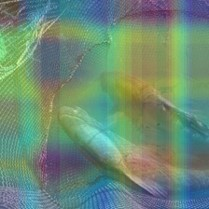
\includegraphics[width=1.2in, height=1.in]{Axial1.jpg}
	                                        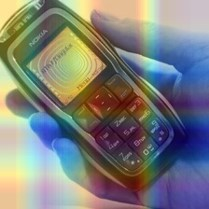
\includegraphics[width=1.2in, height=1.in]{Axial3.jpg}
	                                        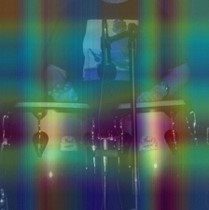
\includegraphics[width=1.2in, height=1.in]{Axial4.jpg}
	                                        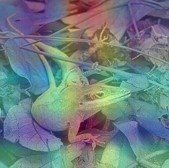
\includegraphics[width=1.2in, height=1.in]{Axial5.jpg}
	                                        }\\
	\subfloat[Squeeze-enhanced Axial attention heatmaps]{\label{heatmap_vis_sea}   
	                                        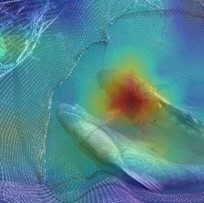
\includegraphics[width=1.2in, height=1.in]{Sea1.jpg}
	                                        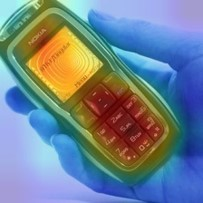
\includegraphics[width=1.2in, height=1.in]{Sea3.jpg}
	                                        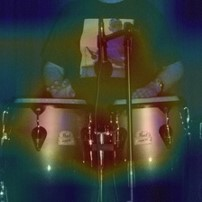
\includegraphics[width=1.2in, height=1.in]{Sea4.jpg}
	                                        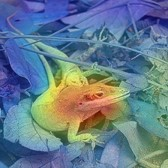
\includegraphics[width=1.2in, height=1.in]{Sea5.jpg}
	                                        }\\	
	\centering
	\caption{The visualization of attention heatmaps from the model consisting of squeeze Axial attention without detail enhancement (\textit{first row}) and SeaFormer (\textit{second row}). Heatmaps are produced by  averaging channels of the features from the last attention block, normalizing to [0, 255] and up-sampling to the image size.}

	\label{heatmap_vis}
\end{figure*}